\documentclass[a4paper,12pt]{article}
\usepackage[T1]{fontenc}
\usepackage{polski}
\usepackage[utf8]{inputenc}
\usepackage[french,polutonikogreek,polish]{babel}
\usepackage{latexsym}
\usepackage{subfig}
\usepackage{graphicx}
\usepackage{sidecap}
\usepackage{wrapfig}
\frenchspacing

\begin{document}

\begin{titlepage}
\title{OBRAZY II - sprawozdanie}
\author{Michał Buszkiewicz, Rafał Mossakowski}
\date{20 XI 2014}
\maketitle
\end{titlepage}

\section{Wprowadzenie}
Celem naszego projektu było stworzenie oprogramowania ułatwiającego komunikacją człowieka z komputerem. Jego działanie opiera się na sterowaniu pozycją kursora w komputerze przy wykorzystaniu ruchów i gestów dłoni użytkownika. Do wykrycia obrazu posłużyła kamera dołączona do komputera oraz odpowiednie metody wchodzące w skład popularnej biblioteki do rozpoznawania obrazów - openCV. Wykonując odpowiednie gesty - np. poruszając otwartą lub zaciśniętą w pięść dłonią, użytkownik moze wydawać polecenia zmiany pozycji kursora lub kliknięcia. Tego typu rozwiązanie technologiczne mogłoby doprowadzić do powstania innowacyjnych interfejsów komputerowych, niewymagających urządzeń wskaźnikowych takich jak myszka czy touchpad.

\section{Wykorzystane techniki}
W związku z dużą ilością możliwych technik wykrywania dłoni oraz gestów na obrazie przesyłanym przez kamerę, byliśmy zmuszeni dokonać wyboru najwydajniejszej z nich na drodze eksperymentu. Po serii prób i błędów postawnowilismy wykorzystać metodę kaskadowych klasyfikatorów Chaara. Metoda ta opiera się na porównywaniu poszczególnych klatek odbieranego strumienia danych ze spacjalnym wzorcem, zawartym w pliku XML. Zastosowane zostały dwa różne wzorce: dla otwartej oraz dla zaciśniętej dłoni. Na obrazie wyświetlanym przez program, wykryte wzorce są oznaczane odpowiednio białym lub zielonym kwadratem. Ponadto, w specjalnym buforze przechowywana jest informacja, mówiąca czy w ostatnich dziesięciu klatkach wykryto otwartą czy zaciśniętą dłoń. Na podstawie jego zawartości podejmowane są odpowiednie akcje zdefiniowane w programie.



\section{Odrzucone techniki}
\subsection{Oddzielenie ręki przez progowanie}
Technika oddzielenia kształtu ręki przez progowanie jest ściśle powiązana z metodami służącymi do wykrycia krawędzi. Obraz wejściowy jest przetwarzany na skalę szarości - zgodnie z wymaganiami metod wykrywania krawędzi biblioteki openCV - po czym zostaje rozmyty z użyciem metody Gaussa w celu usunięcia zbędnych szumów, związanych z niską jakością obrazu. Następnie zostaje zastosowana metoda tzw. tresholdingu, czyli progowania. W efekcie uzyskiwany jest czarno-biały obraz, na którym wyraźnie widnieją kontury ręki. Po wykryciu wspomnianych konturów, obliczany jest związany z nimi centroiod. Zmiana położenia centroidu wskazuje na przesunięcie położenia ręki, co przekłada się na zmianę pozycji kursora. 
Przyczyną odrzucenia tego rzowiązania był fakt, iż jest ono mocno uzależnione od oświetlenia, w którym znajduje się kaera. Pinadto każdy obiekt widziany przez kamerę, niebędący jednocześnie ręką, ma negatywny wpływ na wykrywanie krawędzi - powoduje np. wykrycie "nieistniejących krawędzi".  
\begin{figure}
\centering
\subfloat[obraz wejściowy]{\label{odnosnik}
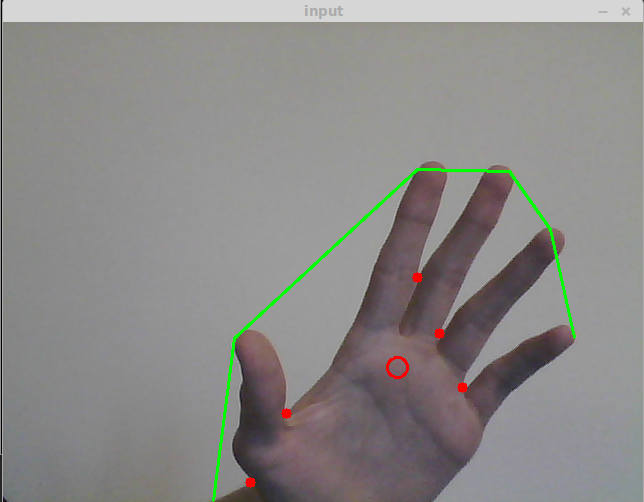
\includegraphics[width=0.45\textwidth]{sprawko_KCK1}}
\quad
\subfloat[obraz progowany]{\label{odnosnik}
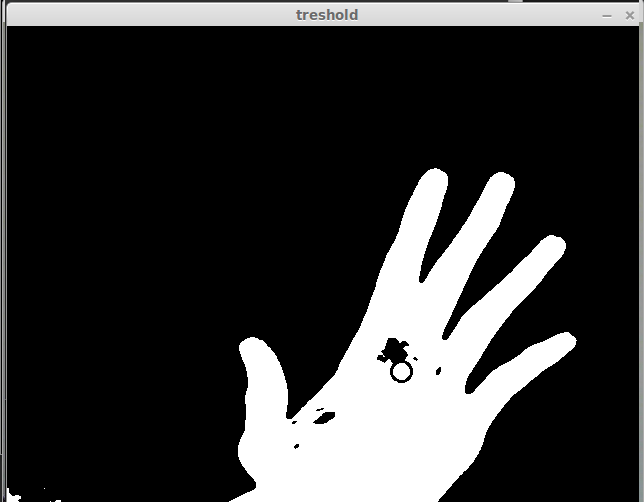
\includegraphics[width=0.45\textwidth]{sprawko_KCK2}}
\caption{Wykryeanie ręki przez progowanie obrazu}
\label{fig:animals}
\end{figure}

\subsection{Metoda próbkowania kolorów ręki}
Metoda próbkowania kolorów ręki jest metodą dwuetapową. W pierwszym etapie, użytkownik proszony jest o umiejscowienie ręki tak, aby była ona widoczna w specjalnym "kwadracie" zaznaczonym w oknie programu. Odpowiedni algorytm "próbkuje" wtedy kolor ręki. Po odpowiedniej kalibracji, program przechodzi do drugiego etapu, polegającego na zaznaczeniu konturów każdego elementu o kolorze podobnym do odczytanego koloru skóry użytkownika. W efekcie prowadzi to do zaznaczenia obszaru dłoni, co umożliwia dalsze sterowanie systemem komputerowym. Niestety rozwiązanie to jest obarczone pewnymi wadami. Największą z nich jest fakt, iż oprócz dłoni, zaznaczana jst także np. twarz użytkownika. Ponadto zmiana oświetlenia w trakcie pracy programu, może prowadzić do niezgodności pobranego początkowo wzorca koloru ludzkiej skóry z rzeczywistym odczytywanym kolorem.


\section{Implementacja}

\end{document}